%Use Lualatex for interpretation!
% lualatex -interaction=nonstopmode --shell-escape UserDocumentation.tex

%You have to have those fonts in your system:
% - Calibri (standard windows font)
% - Trebuchet MS (standard windows font)
% - GROTESKIA (http://www.dafont.com/groteskia.font)

\documentclass[12pt,a4paper]{report}

%\usepackage[utf8]{inputenc} % for old latex interpreters
%\usepackage[english]{babel}

\usepackage{polyglossia}
\setdefaultlanguage[variant=american]{english} % or ?british
\setotherlanguage{czech}

\usepackage{geometry}
\usepackage[cmyk]{xcolor}
\usepackage{amsmath}
\usepackage[some]{background}
\usepackage{listings}
\usepackage{footmisc}
\usepackage{titlesec}
\usepackage{fontspec}
\usepackage{epstopdf,epsfig} 
\usepackage{enumitem}
\setlist[description]{leftmargin=\parindent,labelindent=!}

\definecolor{TextanDarkRed}{cmyk}{.37,.94,.83,.59}
\definecolor{TextanRed}{cmyk}{.0,.879,.844,.220}
\definecolor{javagreen}{rgb}{0.25,0.5,0.35}

\newfontfamily\chapterfont{GROTESKIA}
\newfontfamily\sectionfont{Trebuchet MS}
\titleformat{\chapter}{\chapterfont\fontsize{36pt}{1pt}\selectfont\color{TextanRed}}
  {\thechapter}{20pt}{\chapterfont\fontsize{36pt}{1pt}\selectfont\MakeUppercase}
\titlespacing{\chapter}{0pt}{0pt}{20pt}
\titleformat*{\section}{\LARGE\sectionfont\color{TextanDarkRed}}
\titleformat*{\subsection}{\fontsize{14pt}{1pt}\selectfont\sectionfont\itshape\color{TextanDarkRed}}\titleformat*{\subsubsection}{\sectionfont\color{TextanDarkRed}}

\setmainfont{Calibri}

\backgroundsetup{
scale=1,
angle=0,
opacity=1,
contents={
\begin{tikzpicture}[remember picture,overlay]
  \path [fill=TextanDarkRed] (-0.5\paperwidth,-0.5\paperheight)rectangle (-0.37\paperwidth,0.5\paperheight);
 \end{tikzpicture}}
}

\usepackage[unicode,colorlinks=true]{hyperref}
\hypersetup{pdftitle=TextAn - user documentation}
\hypersetup{pdfauthor={Petr Fanta, Duc Tam Hoang, Adam Huječek, Václav Pernička, Jakub Vlček}}
\hypersetup{linkcolor=black, citecolor=black, urlcolor=black, filecolor=black}

\def\chapwithtoc#1{
\chapter*{#1}
\addcontentsline{toc}{chapter}{#1}
}

% sets numbering for subsubsection
\setcounter{secnumdepth}{3}
\setcounter{tocdepth}{3}

\lstdefinelanguage{properties}{% new language for listings
  basicstyle=\ttfamily,
  sensitive=false,
  morecomment=[l]{\#},      % comment
  morestring=[b]",          % string def
  commentstyle=\color{javagreen},
  basicstyle=\small
}

%Comment macro
%Usage:
% \comment[_assignee_]{_author_}{_comment_}
% \comment{_author_}{_comment_}
\makeatletter
\newcommand{\comment}[3][\@empty]{
  {\color{magenta}[#3 - }
  {\color{green}\ifx\@empty#1\relax Author: #2 \else Assignee: #1; Author: #2\fi}{\color{magenta}]}
}
\makeatother

\newcommand{\textan}{\emph{TextAn}}

\begin{document}

\begin{titlepage}
\BgThispage
\newgeometry{left=4.5cm,top=7cm,bottom=3cm}

\begin{figure}
 
\includegraphics{../Logos/TEXTAN_logo_grey_B}
\end{figure}
\noindent
\textcolor{TextanRed}{\chapterfont\fontsize{48pt}{1pt}\selectfont\MakeUppercase{User documentation}}\\[15pt]
\textcolor{TextanDarkRed}{\sectionfont\LARGE\MakeUppercase{Version 0.1}}

\vfill
\noindent
\begin{minipage}[b]{.75\textwidth}
\textbf{Authors}\\
Petr Fanta\\
Duc Tam Hoang\\
Adam Huječek\\
Václav Pernička\\
Jakub Vlček
\end{minipage}% This must go next to `\end{minipage}`
\begin{minipage}[b]{.25\textwidth}
\textbf{Supervisor} \\
Ondřej Bojar\\
%\vfill
\\
\\
\textbf{Date}\\
\today
\end{minipage}

\end{titlepage}
\restoregeometry

\pagenumbering{roman}
\tableofcontents

%\chapter*{Intro}
%\addcontentsline{toc}{chapter}{Intro}

\chapter{User Guide}
\pagenumbering{arabic}

\section{Introduction}
% Section: Introduction

% FOR ENTERTAIN: The spider opens his heavy eyes. He stand up, look through the lousy windows. The sun is flaring, kissing all over the earth. He said to himself: ``It's time''. Students are rushing out of the dormitory like rats desert from a sinking ship. Some are going to the public transport, waiting for the regular hooves from the distance. The bus comes and goes, its double tires sing high notes on the road. Some are visiting the car park. The wheels of the cars creaked around, then they crawled into the city centre. A man and girl are crossing street, with their arms around each other's waists. Then the man must have said something supposed to be funny because two of them are laughing like hyenas. The spider retreats from the windows. The daily screen makes him so lonesome and depressed. Another day has just begun.

%TODO what is textan

%TextAn (Text Analyser) is the product of our software project groups (consists of 5 members) at Faculty of Mathematics and Physics, Charles University in Prague (MFF UK). The tool is attributed to Software Project subject, developed in 9 months from Jan 2014 to Sep 2014, and supervised by RNDr. Ondřej Bojar, PhD. It is a client-server tool which support mining structured information from text documents. At the moment, the documents are specified to police report but TextAn could be applied to a wide range of domains. 

% --> to DeveloperDocumentation
% 

%TODO basic usage

\comment{Adam}{Add something here!}

\subsection{System overview}

%What is this?

%what textan do, something which is 

%WHAT DOES THE POLICE WANT? OF COURSE NOT ARREST US

% 

% it should be something better, for example, what textan to in a : What textan to. what you can expect in the rest of documentation . If you don't need what we offer in textan, leave a comment and get away.

\comment[Jakub]{Adam}{Ondrej had a lot of comments on introduction, but if you
are about to change it completely, I will not bother to translate them, unless
you explicitly ask for them.}

With the profiliferation of unstructured written texts, the need for a tool to mine the structure out of such documents is on increasing trend. 
\textan{} (Text Analyser) serves such purpose, targeting the Police reports. 
In other words, \textan{} is a tool which supports mining structured data buried in the Police reports. The term "structured data" consists of two concepts. 
First, it contains name, street, date of birth, crime and other named entities related to some people. 
Second, the data contain the relations between two entities. 
For example, the relation between a person and their date of birth, the relation between two persons. The objective of \textan{} is to provide a robust tool which supports the procedure, either automatically and manually.
Although first impulse came from the Police needs, \textan{} is made as general
as possible to allow easy configuration for any other domain as needed.

\textan{} has client-server structure. It supports following operations:
  
  \begin{itemize}
  \item Bring new solution to the classic problem of extracting data from text.
  \item Provide the service for both automatic detection and manual adjustment.
  \item Make the adjustment of data as simple as possible for users.
  \item Make the graphic user interface as fruitful as possible.
  \end{itemize}

This documentation describes \textan{} from the perspective of an user. 
All the concepts are explained in the \emph{Glossary}.

To start using \textan{}, user have to start the client application and log in. 
Once user log in successfully, the main screen of \textan{} is displayed.

\comment{Tam}{What's next?} 
\comment{Adam}{The last paragraph is not needed IMO.}

\subsection{Glossary}
Terms are used in very specific manner in the documentation and in both the
client and the server, therefore it is really essential to understand their
meaning. Otherwise, it is possible to misunderstand the rest of the text.

\comment[anyone]{Petr}{check if this makes sense!}
\begin{description}
\item[Document]
The document is an arbitrary text that is processed by \textan{}. E.g. a police
report, a letter, a movie review or a judgment. In the following text the terms
document and report are used interchangeably.

\item[Object]
The term "object" refers to our representation of some unique thing in
\textan{}. Consider for example a person with name Joseph Smith from Prague with
identifier 000123/4567. The object refers to this person in the real world, in
meat and bones.

\item[Alias]
The alias represents a designation of a object. For example: Joseph Smith, Joe
Smith, Joey S., J. Smith or just Smith can be names of one concrete person.
Names are aliases for the person.

\item[Entity]
An entity is a sequence of words recognized either by a named entity recognizer
or by a user. \comment[Petr]{Petr}{Move to next paragraph - Object assigment}
The entity will be later assigned to an object and it becomes an alias
of the object. Consider for example the sentence: Joe Smith was seen
in Prague on 5th September. The sentence contains 3 entities: Joe Smith (person),
Prague (city), 5th September (date). We don't know which objects belong to these
entities yet. Prague can represent the capital city of the Czech Republic,
or a city in the USA.

\item[Object/Entity Type]
Each object and each entity has a type. For example person, date, city, country
etc. The set of types in the system depends on the domain which the system is
deployed to.

\item[Object Assigment]
\comment[Petr]{Petr}{Description of object assigment}

\item[Alias occurrence]
\comment[Petr]{Petr}{Description of alias occurence}

\item[Object Merging]
\comment[Petr]{Petr}{Description of object merging}

\item[Relation]
The relation represents any relationship between objects mentioned in a document.
A relation can be represented in a document by an anchor word, or it can be
unexpressed, which means without any anchor in a document. See Anchor below.
\comment[anyone]{Adam}{Check this sentence with two relations, one with anchor, one without anchor.}
Consider this example: "Adam (890524/1367) is married to Eve". Three objects
appear in the sentence - persons Adam and Eve and the id 890524/1367. There
are two relations: Adam "has" 890524/1367 without an anchor and Adam "marriage"
Eve with the anchor "married".

\item[Relation Type]
Each relation has a type. For example born, reside, die, kill etc. Similarly to
object/relation types the set of relation types in the system depends on the
domain which the system is deployed to.

\item[Anchor]
An anchor is a word or a sequence of words that is bound to a relation between
objects. Consider for example the sentence: Joey Smith killed Mary-Ann S. There
is a relation between Joey Smith and Mary-Ann S., which is represented by the
word "killed". The word is the anchor. \comment{Ondrej}{Why do you not write
about type here?}

\item[Roles and orders]
Each object in a relation can have a role assigned. This role is mostly used
for visualisation and storing additional information. Moreover object can also
have order assigned which is just an integral number used for graph
visualization\ifdefined\USRDOC{} (see Section \ref{sssec:EditRelations})\fi{}
\ifdefined\DEVDOC{} (see Section \ref{USR-sssec:EditRelations} in the user
documentation)\fi{}. For example relation created from sentence
"Bill killed Joe." could be represented like this:
Bill (-1, murderer) --kill--> (1, victim) Joe.
\end{description}




\section{Client Usage}
% Section: Client Usage
This section contains all information needed by end users to successfully use
the \textan{} client application. For instructions to actual run the client
see Section \ref{sssec:StartClient}. \comment{Ondrej}{I do not understand what
will be there, why chapter 2 and not sooner?}

\subsection{First Run}

On the first run of \textan{} client, users are prompted to enter their username
(see figure \ref{fig:Login}, which is used by the system to identify the users.
The login name is stored in settings and the login dialog is not shown again
in following runs. The name can be changed in settings (see Section
\ref{ssec:Settings}). A valid name is required, ie. not empty and not whitespace
characters only. If users enter invalid login, a warning is displayed and they
may enter other login or the application quits.

\begin{figure}[!htb]
        \centering
        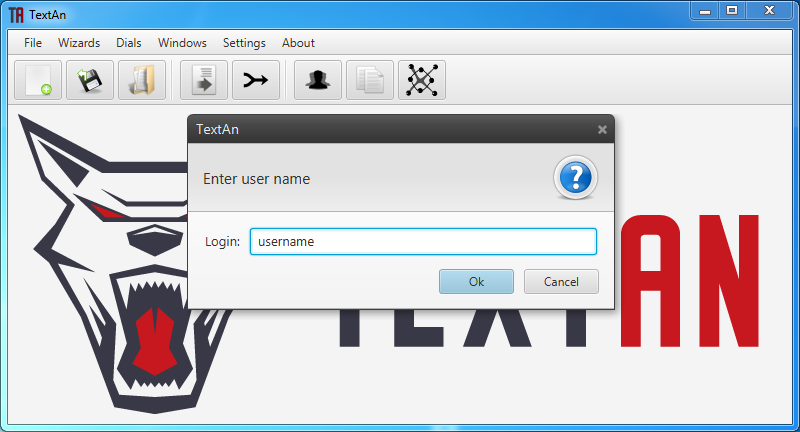
\includegraphics[width=\textwidth]{Images/login}
        \caption{Login prompt on first run.}
        \label{fig:Login}
\end{figure}

\subsection{Working Space}

The \textan{} client's application working space is very simple and intuitive.
The main window (see Figure \ref{fig:MainWindow}) contains the main menubar with
all commands needed to control the application. There is also a toolbar with
icons for mostly used commands to speed up the access. Hover over the
toolbar icons to see the corresponding action names.

\begin{figure}[!htb]
        \centering
        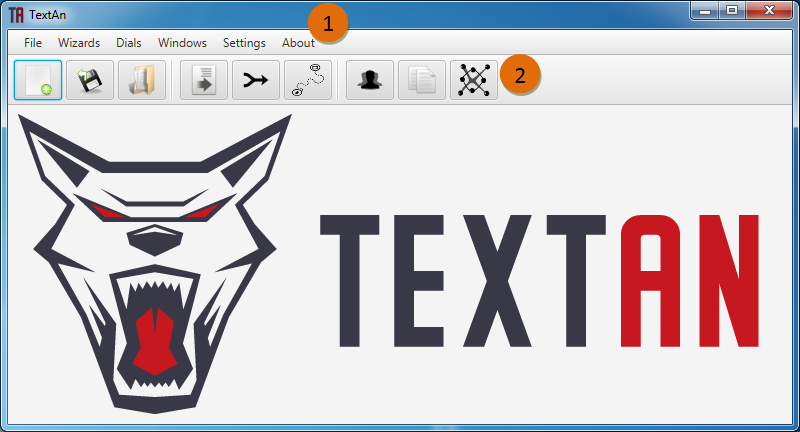
\includegraphics[width=\textwidth]{Images/main}
        \caption{Main window controls. 1) Main menubar, 2) Toolbar.}
        \label{fig:MainWindow}
\end{figure}

The File menu contains items to create new report, import report from external
file and load report whose processing was not finished, but was saved to continue
later. For more information about report processing, see Section \ref{ssec:ProcessReport}.

The Wizards menu contains items starting wizards to guide the users in more
complicated tasks, like processing report (see Section \ref{ssec:ProcessReport})
and joining objects (see Section \ref{ssec:JoinObjects}).

The Dials menu contains items to display objects, documents and relations
stored in the database (see Section \ref{ssec:ViewDatabase}).

The Windows menu contains the list of currently displayed application windows
to easily bring certain window to front.

The Settings menu contains items to customize \textan{} client appearance and
behavior. For more information, see Section \ref{ssec:Settings}. It also
contains shortcut to reset the position and size of the main window.

\subsection{Settings}
\label{ssec:Settings}

This section describes options available in individual items contained in the
main menu Settings.

\subsubsection{General Settings}
\label{sssec:GeneralSettings}

The General Settings window (see Figure \ref{fig:GeneralSettings}) contains
controls for changing the behavior and appearance of the application.

\begin{figure}[!htb]
        \centering
        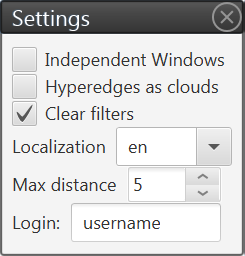
\includegraphics{Images/general}
        \caption{General Settings Window}
        \label{fig:GeneralSettings}
\end{figure}

\paragraph{Independent Windows} If this control is checked, the application
secondary windows will not be embedded into the main window, but separate
independent system windows will be used.

\paragraph{Hyperedges as clouds} This control affects the rendering of
hyperedges\footnote{Hyperedge is an edge in a hypergraph which is a
generalization of term graph. The difference is that edges in hypergraphs can
connect any number of nodes, whereas in graph they always connect two nodes.}
in graphs (see Figure \ref{fig:Hypergraphs}). The default rendering transforms
hypergraphs to graphs by adding auxiliary nodes of square shape representing
the relation. If this control is checked, the edges are rendered by graph
background.

\begin{figure}[!htb]
        \centering
        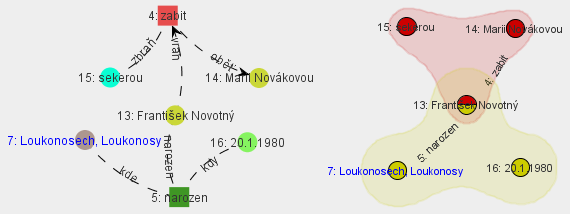
\includegraphics[width=\textwidth]{Images/hypergraphs}
        \caption{Graph rendering differences. Default on the left.}
        \label{fig:Hypergraphs}
\end{figure}

\paragraph{Clear Filters} If this control is checked, the filter fields
displayed during report processing will be cleared when shown again.

\paragraph{Localization} This control determines the language of the \textan{}
client. The Czech and English localizations are currently supported. The
default language is English. Changing localization takes effect after
restarting the application.

\paragraph{Max Distance} This control affects the default maximal length of the
path between any node and the graph central node. Nodes beyond this limit are
not displayed.

\paragraph{Login} This control enables users to change their username. Changing
login takes effect after restarting the application.

\subsubsection{Colors}
The Colors settings window (see Figure \ref{fig:Colors}) contains two lists -
one for object types and one for relation types. They contain all types found
in the database and enable users to easily customize their color displayed in
graphs views and report processing windows by clicking corresponding color
pickers.

\begin{figure}[!htb]
        \centering
        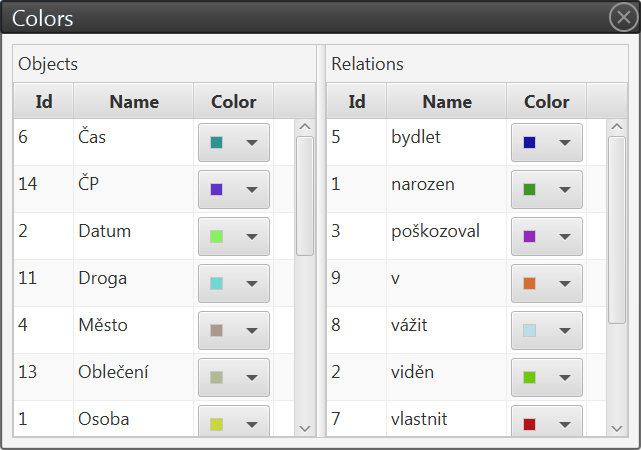
\includegraphics[width=\textwidth]{Images/colors}
        \caption{Colors settings window.}
        \label{fig:Colors}
\end{figure}

\subsection{Report Processing}
\label{ssec:ProcessReport}

The wizard for report processing is accessible from the main menu. It guides
users in complicated procedure of processing a report. The procedure is divided
into several steps described in this section (see figure \ref{fig:Pipeline}).
Users can return to previous steps, but if any changes are done, the progress
in following steps is lost.

\begin{figure}[!htb]
        \centering
        
\includegraphics[height=16cm,keepaspectratio]{Images/pipeline}
        \caption{Schema of report processing.}
        \label{fig:Pipeline}
\end{figure}

In Edit Report step and later, when the report processing is interrupted,
\textan{} offers to save the unfinished report into a file. The processing can
be resumed by selecting Unfinished Report in Report Source step (see Section
\ref{sssec:ReportSource}). The processing continues in the step where it was
saved.

\subsubsection{Report Source}
\label{sssec:ReportSource}

\begin{figure}[!htb]
        \centering
        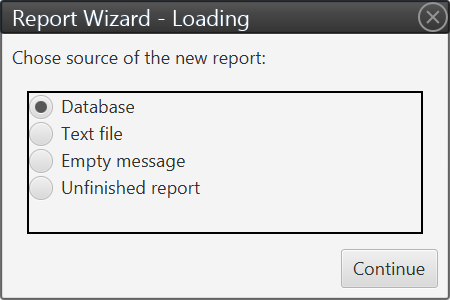
\includegraphics{Images/source}
        \caption{Choosing report source.}
        \label{fig:Source}
\end{figure}

This step (see figure \ref{fig:Source}) allows users to choose the source of the
report. The following sources are possible:

\paragraph{Database} This option displays (see figure \ref{fig:Database}) list
of all unprocessed reports stored in the database (for filtering details see
Section \ref{sssec:DocumentList}).
The report cannot be edited, so the wizard then proceeds to Edit Entities step
(see Section \ref{sssec:EditEntities}). \comment[Adam]{Ondrej}{The following is
not completely comprehensible} If the report is edited by someone else
externally while being processed by a local user, a warning message is
displayed. The local user can decide whether the report processing should end or
continue with the current text. In the latter case, the current text overwrites
the one in the database when processed report is saved to the database. It is
also possible to enter Edit Report step and edit it as it will replace stored
text anyway.

\begin{figure}[!htb]
        \centering
        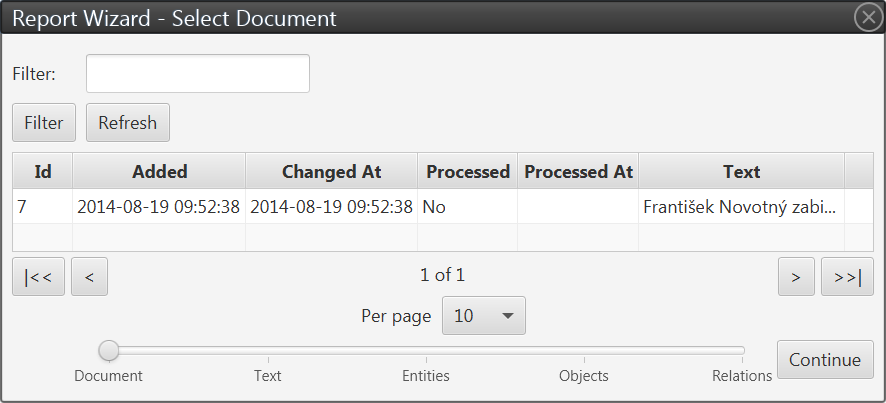
\includegraphics[width=\textwidth]{Images/database}
        \caption{Chosing report from database.}
        \label{fig:Database}
\end{figure}

\paragraph{Text File} This option displays open file dialog for importing
report text from external file. The extracted text is then displayed (see
Figure \ref{fig:TextFile}, so users can chose the proper file encoding. Then
the wizard proceeds to Report Edit step (see Section \ref{sssec:ReportEdit}).

\begin{figure}[!htb]
        \centering
        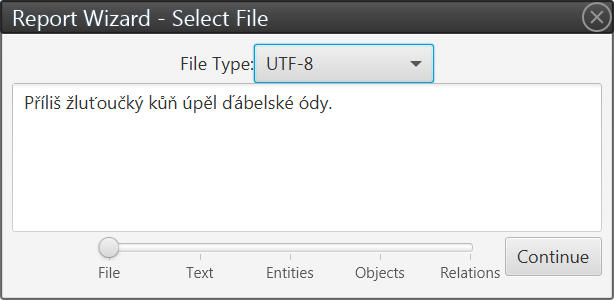
\includegraphics[width=\textwidth]{Images/textfile}
        \caption{Chosing encoding of the file.}
        \label{fig:TextFile}
\end{figure}

\paragraph{Empty Message} This option proceeds directly to Report Edit step
(see Section \ref{sssec:ReportEdit}) with empty report.

\paragraph{Unfinished Report} This option displays open file dialog for
selecting the file with report whose processing has not been finished, but it
was stored to continue later. The wizards then proceeds to step where report
processing has been interrupted.

\subsubsection{Edit Report}
\label{sssec:ReportEdit}

In this step users can edit the text of the report (see Figure
\ref{fig:ReportEdit}. This step is followed by Edit Entities step (see Section
\ref{sssec:EditEntities}).

\begin{figure}[!htb]
        \centering
        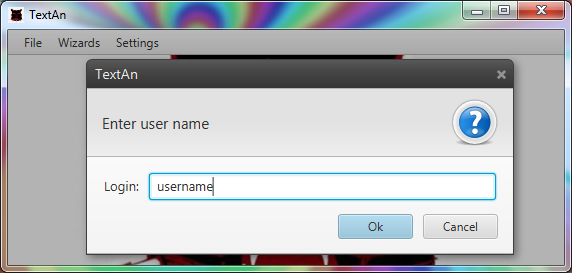
\includegraphics[width=\textwidth]{Images/reportedit}
        \caption{Editing the text of the report.}
        \label{fig:ReportEdit}
\end{figure}

\subsubsection{Edit Entities}
\label{sssec:EditEntities}

Before entering this step the system automatically recognizes named entities
in the report text. Recognized entities are marked by text color. Entities of
the same type have the same color (see Figure \ref{fig:Entities}). Hovering over
entity text will display its type.

Users can correct recognized entities and add new ones by selecting the text
of the entity by mouse and picking the entity type from the context menu.
There is a filter field in the context menu to allow users enter substring of
name of the desired entity type to speed up the selection process. If there are
only one item in the list left, it can be selected by pressing enter too.
Pressing Down key in the filter field transfers focus to the list, so keyboard
keys Up, Down and Enter can be used to select the entity type.

One entity cannot comprise from several separated parts and entities cannot
overlap.

This step is followed by Edit Objects step (see Section
\ref{sssec:EditObjects}).

\begin{figure}[!htb]
        \centering
        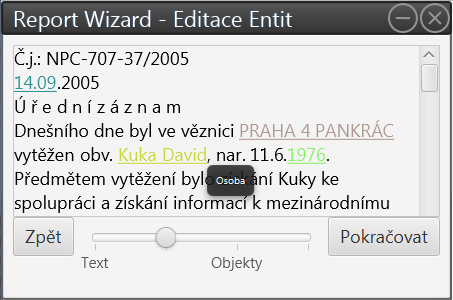
\includegraphics[width=\textwidth]{Images/entities}
        \caption{Editing entities in the report.}
        \label{fig:Entities}
\end{figure}

\subsubsection{Edit Objects}
\label{sssec:EditObjects}

In this step the entities are assigned to real objects (see Figure
\ref{fig:Objects}). The system automatically assigns objects stored in the
database to entities recognized in the database. If no suitable object is
found, the entity is marked with orange background. Hovering over entity
displays its type and assigned object if any.

\begin{figure}[!htb]
        \centering
        
\includegraphics[width=\textwidth]{Images/objects}
        \caption{Editing objects in the report.}
        \label{fig:Objects}
\end{figure}

Right click on objects will display context menu with options to show the graph
of the object or documents containing the object. This is also true for all following steps.

To assign object to entity left click the entity and select suitable object
from the context menu (see Figure \ref{fig:ObjectMenu}) or create entirely new
object.

\begin{figure}[!htb]
        \centering
        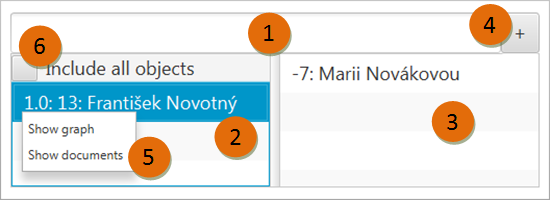
\includegraphics[width=\textwidth]{Images/objectmenu}
        \caption{Menu for selecting object. 1) Filter field, 2) List of
		 recommended objects (with probability of match), if 6) is checked, list
		 of objects of given type from database, 3) List of new objects created
		 during editation of the same type, 4) Button for creating new object,
		 5) Menu for more information about the object.}
        \label{fig:ObjectMenu}
\end{figure}

The report processing cannot continue unless all entities have assigned
objects. This step is then followed by Relation Edit step (see Section
\ref{sssec:EditRelations}).

\subsubsection{Edit Relations}
\label{sssec:EditRelations}

This is the last mandatory step during report processing (see Figure
\ref{fig:Relations}). It consists of marking relationships between objects in
the document.

\begin{figure}[!htb]
        \centering
        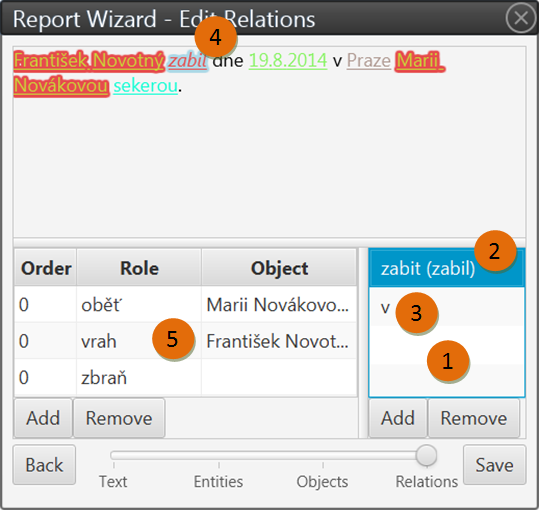
\includegraphics[width=\textwidth]{Images/relations}
        \caption{Editing relations in the report. 1) Relation list, 2) Relation
		 with anchor, currently selected, 3) Relation without anchor, 4) Highlighted
		 relation anchor, note highlighted objects too, 5) Objects assigned to
		 the selected relation}
        \label{fig:Relations}
\end{figure}

Relation with anchor can be created by selecting the words of the anchor by
mouse and picking a relation type from context menu. Empty relation with given
anchor and type is added to the list of relations. Empty relation without anchor
can be added by Add button under the relation list and picking a relation type
from dialog. New relations will have prefilled some roles based on relations of
that type already stored in the database. Selecting a relation in the relation
list highlights its anchor and assigned objects.

To add an object to a relation, select the relation in the list of relations.
Use Add button under object list to add new row to the object table. Double
clicking the object cell opens combobox with the list of objects in the report
to assign to the relation. Or you can drag the object from the report text and
drop it to empty row or Add button to add new row. Dropping the object into the
non empty row replaces the assigned object. Any string can be specified as
a role. If any roles exist for the relation in the database, combobox with
is displayed for the role column.

Order column effects displaying arrows in the graph views. For binary
relations the arrow points from object with negative order at object with
nonnegative order. For relations with more than two objects assigned, arrows
point from objects with negative order and at objects with positive odd order.

After finishing relation editation the document is stored to the database,
unless some errors occur. In that case Error Step follows (see Section
\ref{sssec:Errors}).

\subsubsection{Errors}
\label{sssec:Errors}

This step takes place only if some changes to the database from other sources
are detected (see Figure \ref{fig:Errors}). The window informs user which new
objects and relations have been created while the report was being processed and
which objects have been joined. Users can decide to return to previous steps
and reconsider their edits or force the saving of the report.

\begin{figure}[!htb]
        \centering
        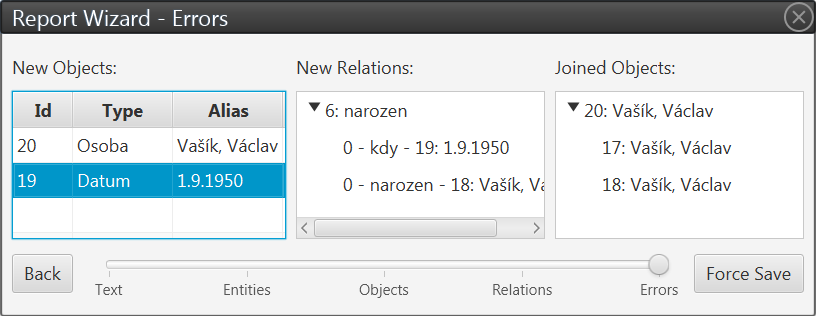
\includegraphics[width=\textwidth]{Images/errors}
        \caption{Errors when saving report.}
        \label{fig:Errors}
\end{figure}

\subsection{Database Exploration}
\label{ssec:ViewDatabase}

Users can use client to view data stored in the database by selecting items
in Dials menu of the main window. Other ways include various context menus
while processing reports etc.

\subsubsection{Browsing Objects}
\label{sssec:ObjectList}

This window contains list of objects matching the filter criteria (alias text,
object type) paginated for more convenient work (see Figure
\ref{fig:ObjectList}. Please note that changing filter criteria must be confirmed by pressing Filter button. Use right mouse button click to open context menu for displaying graph for the selected object (see Section \ref{ssec:Graphs}) or for displaying list of documents containing it (see
Section \ref{sssec:DocumentList}).

\begin{figure}[!htb]
        \centering
        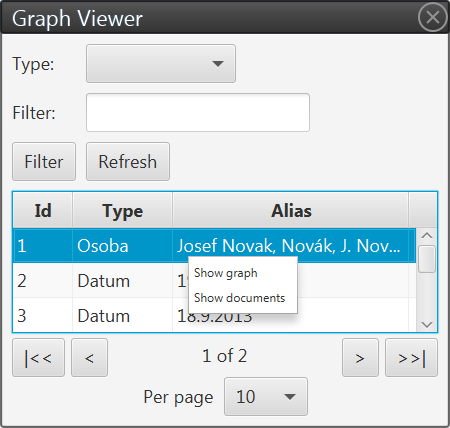
\includegraphics{Images/objectlist}
        \caption{List of objects.}
        \label{fig:ObjectList}
\end{figure}

\subsubsection{Browsing Documents}
\label{sssec:DocumentList}

This window contains list of documents matching filter criteria. Please note
that not all filter controls may be visible at all situations as they are
customized to fit the current context (see Figure \ref{fig:DocumentList}.
Also note that changing filter criteria must be confirmed by pressing Filter
button. Use right mouse button click to open context menu for displaying graph
for the selected document (see Section \ref{ssec:Graphs}) or for displaying the
report itself (see Section \ref{sssec:DocumentView}). Other options include
editing the report or processing it if possible. Inserting new report without processing is done by clicking New document button. Hovering over the row displays full report text.

\begin{figure}[!htb]
        \centering
        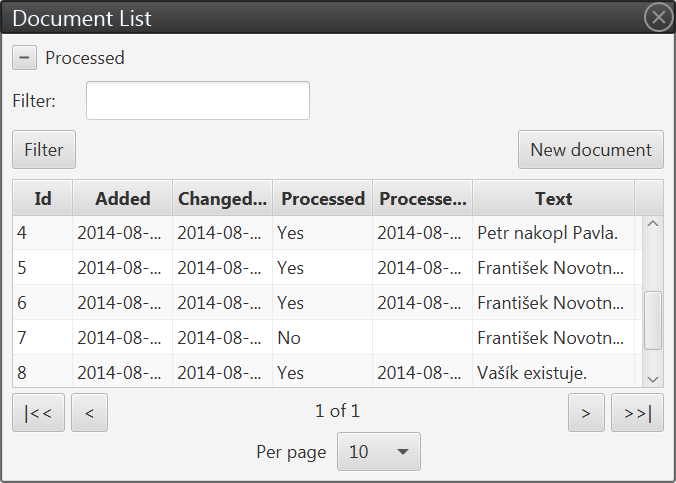
\includegraphics[width=\textwidth]{Images/documentlist}
        \caption{List of documents.}
        \label{fig:DocumentList}
\end{figure}

\subsubsection{Browsing Document}
\label{sssec:DocumentView}

This window displays reports with highlighted objects and relations for easier
orientation (see Figure \ref{fig:DocumentView}). Use right mouse click to open
object context menu to get more information about the selected object. Selecting
relation will highlight its anchor and assigned objects.

\begin{figure}[!htb]
        \centering
        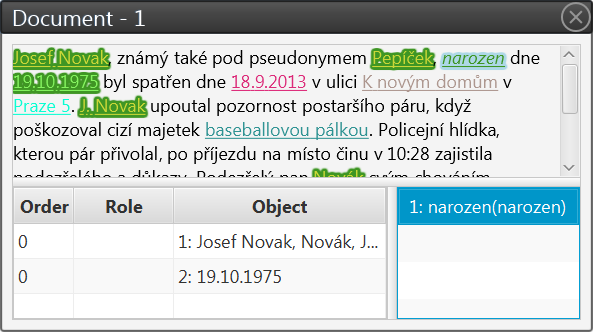
\includegraphics[width=\textwidth]{Images/documentview}
        \caption{Document detail.}
        \label{fig:DocumentView}
\end{figure}

\subsubsection{Browsing Relations}

This window contains list of relations matching the filter criteria (anchor
text, relation type) paginated for more convenient work (see Figure
\ref{fig:RelationList}). Please note that changing filter criteria must be
confirmed by pressing Filter button. Use right mouse button click to open
context menu for displaying graph for the selected relation (see Section
\ref{ssec:Graphs}) or for displaying list of documents containing it (see
Section \ref{sssec:DocumentList}).

\begin{figure}[!htb]
        \centering
        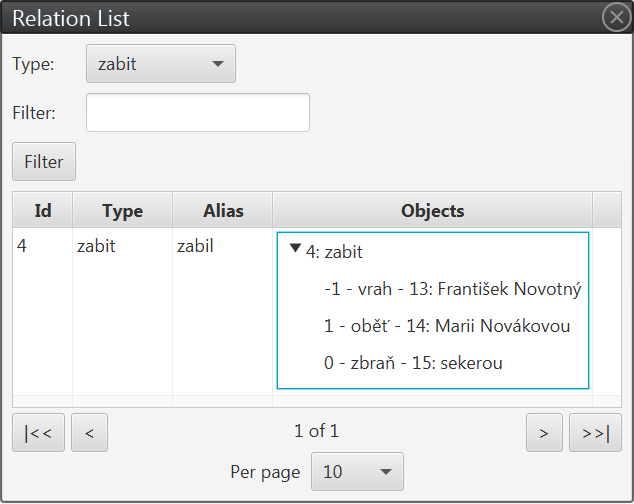
\includegraphics[width=\textwidth]{Images/relationlist}
        \caption{List of relations.}
        \label{fig:RelationList}
\end{figure}

\subsection{Graph Views}
\label{ssec:Graphs}

Graph Windows can be displayed from many places in \textan{} client. Most
common way is right clicking an object/relation/document and selecting Show
graph context menu item.

The graph appearance is drastically effected by Hypergraphs settings (see
Section \ref{sssec:GeneralSettings}).

In the top part of the window (see Figure \ref{fig:Graph}) there is a toolbar
with icons to manipulate the graph.

The first icon represents Transformation and is used to manipulate the graph as a whole, eg. panning or rotating (hold CTRL while left clicking and moving the
mouse). The second icon represents Picking and is used to manipulate subset of
nodes. Hold left mouse button and drag to select multiple nodes and then click
and drag to move them. The third icon centers the view to graph center.
Distance field can be used to change the "radius" around the central node.
Confirm its editing by clicking Go button. Use mousewheel to zoom the graph.

Nodes representing objects can be right clicked to show context menu with
options to display their surroundings or documents. Right clicking edges or
nodes representing the relations shows context menu for centering to objects
assigned to the relation.

On the sides there are lists of object/relation types to display. Unchecking
the type will cause objects/relations of that type to disappear when graph is refreshed by Go button. Clicking the three dots shows or hides the filter
lists.

\begin{figure}[!htb]
        \centering
        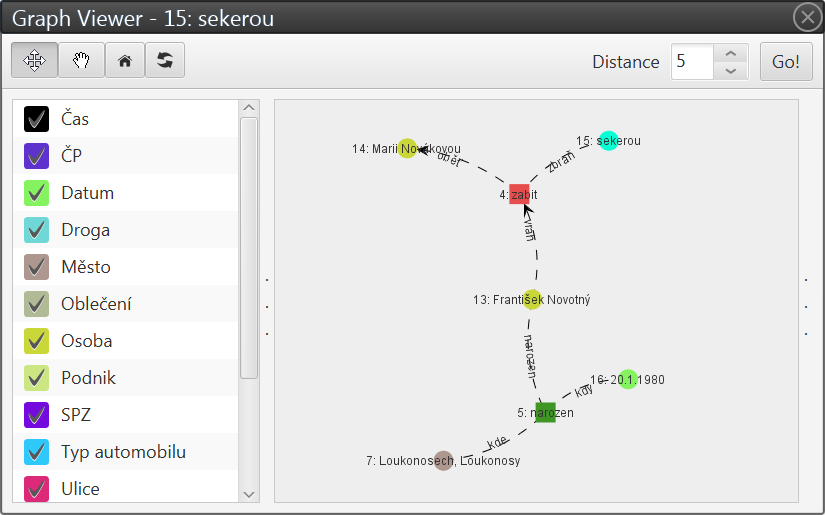
\includegraphics[width=\textwidth]{Images/graph}
        \caption{Graph window.}
        \label{fig:Graph}
\end{figure}

\subsection{Joining Objects}
\label{ssec:JoinObjects}

There can be situations when it is discovered that two objects originally
thought to be independent are in fact one object. For such cases there is Join
Object wizard (see figure \ref{fig:Join}). For more information about object
lists see Section \ref{sssec:ObjectList}.

\begin{figure}[!htb]
        \centering
        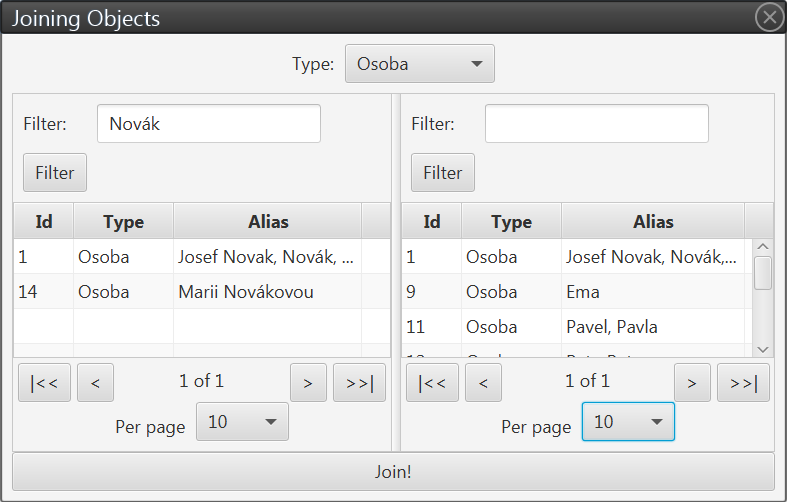
\includegraphics[width=\textwidth]{Images/join}
        \caption{Join Object Wizard.}
        \label{fig:Join}
\end{figure}

The objects to merge must have common type. Select one object in left object
list and the other one in right object list. The button Join will start the
joining itself.

\subsection{Path Wizard}
This wizard displays window similar to Joining Objects. Select two objects
for which you want to try to find path of relations and objects connecting them
(see Figure \ref{fig:Path}). The system looks only for the shortest route.
If such path is found, the graph displaying it is shown.

\begin{figure}[!htb]
        \centering
        
\includegraphics[width=\textwidth]{Images/path}
        \caption{Path Wizard.}
        \label{fig:Path}
\end{figure}

\comment[Adam]{Adam}{Add figure with path graph.}


\chapter{Administrator guide}

\section{Domain and conventions}
% Section: Domain and convention

Because \textan{} is very universal, it is necessary to use right configuration.
\textan{} system can be a really powerful tool, but it must be configured properly
for your domain to achieve the best results. Also it is important to establish
some convention that describes usage of the configuration.

The domain is represented by object types and relation types, eventually by roles
of relation types. \comment[Petr]{Petr}{Example: types for police reports vs types for movie descriptions}

If you define too big set of types, it can be difficult for users to understand
their usage. Otherwise, if you define too small set of types, their meaning will
be vague which could confuse users. It is very difficult to select suitable set
of types.

In addition, every user has his own opinion when to use certain type. In this
situation, it can be useful to define the convention. The convention should contain
explanation how to use each concrete type and examples of usage.


\section{Language}
% Section: Language

Although \textan{} was developed with Czech  as the first supported language
and it is preset for
Czech language by default, it is possible to configure \textan{} for other languages,
especially English. For now, \textan{} assumes that all documents in the dataase
are in a single language. There are
two areas which depend on the selected language: named entity recognition and full
text search. Both of them are placed in the server application along with other
business logic.

The first thing that needs to be re-configured for a new language is {\it
NameTag}, the name entity recognizer. 
You must change property {\it ner\_identifier}
specifying an appropriate tagger and providing
training data in desired language. See Section \ref{sssec:NametagSettings} for
a detailed description.

The second thing, that needs to be configured, is the full text search. The system
internally uses Apache Lucene, full text search engine. Lucene provides creation
of full text indexes and searching in them. To get good results, it is necessary
to perform some preprocessing, such as replacing words with their stems
(stemming), removing stop words or expanding synonyms. This is done through an
Analyzer. Lucene contains Analyzers%
\footnote{\url{http://lucene.apache.org/core/4_7_0/analyzers-common/overview-summary.html}}
for many common languages, or you can define your own. The selection of an Analyzer in 
\textan{} is done through the property \emph{hibernate.search.analyzer} in
\emph{data.properties}. See Section \ref{sssec:DataSettings}.


\section{Web services}
% Section: Web Services
XML-based web services (or W3C web services) are a method of communication in
the client-server model. It means, that the server exposes web API described in
WSDL. This makes developing different clients that can communicate with
\textan{} server very easy.

These WSDL files are available either in source codes, or on URL \emph{http://hostname:port/soap},
where hostname indicates a computer with \textan{} server instance running on the port.

For more information about communication pattern see develeper documentation
section \ref{DEV-sec:Communication}.


\section{Security}
\label{sec:Security}
% Section: Security

By default, the environment is assumed to be completely safe, so no security
measures are in place. However the \textan{} supports encrypted communication
and even client authentication.

For detailed description of individual properties, see Section
\ref{sssec:WebServerSettings} for server configuration and Section
\ref{sssec:BasicConf} for client configuration.

\subsection{SSL}

Enabling secure communication consists of setting several properties, both
on server and client side.

For server the following setting is required. Most importantly \emph{server.ssl} must
be set to \emph{true}. Then these properties will be used by the server:
\emph{server.ssl.keyStore.path} must point to the key store containing
certificate and private key for server to use. Its type is determined by
the content of property \emph{server.ssl.keyStore.type}, default value is JKS.
Property \emph{server.ssl.keyStore.password} specifies password to the key
store and property \emph{server.ssl.keyManager.password} specifies the password
for the private key. Port used for secure communication can be configured by
\emph{server.ssl.port}.

For client the following setting is required. Most importantly property \emph{ssl} must
be set to \emph{true}. Then these properties will be used by the server:
\emph{ssl.trustStore} must point to the trust store containing the certificate
of the server. Its type is determined by the content of property
\emph{ssl.trustStore.type}. Property \emph{ssl.trustStore.password} specifies
password to the trust store.

\subsection{Client Authentication}

For limiting the access to the webservices, client authentication can be turned
on. Only client that provides certificate from authority trusted by the server
will be served.

For server the following setting is required. Most importantly
\emph{server.ssl.clientAuth} must be set to \emph{true}. Then these properties
will be used by the server: \emph{server.ssl.trustStore.path} must point to the
trust store containing certificate of the trusted certificate authority for
server. Its type is determined by the content of property
\emph{server.ssl.trustStore.type}, default value is JKS. Property
\emph{server.ssl.trustStore.password} specifies the password to the trust
store.

For client the following setting is required. Most importantly property
\emph{ssl.clientAuth} must be set to \emph{true}. Then these properties will be
used by the server: \emph{ssl.keyStore} must point to the key store containing
the private key and certificate signed by the certificate authority trusted by
the server. Its type is determined by the content of property
\emph{ssl.keyStore.type}. Property \emph{ssl.keyStore.password} specifies password
to the key store.


\section{Server}
% Section: Server

This section contains all information to successfully install, configure and run
\textan{} server side application.
\comment[anyone]{Petr}{add short introduction for this section, remind configuration
options, complexity atc.}

\subsection{Installation guide}

This section describes how to install and configure \textan{} server on a server
machine.

\subsubsection{Prerequisites}
\label{sssec:SerInstPre}

The \textan{} server requires installation of \emph{Java 8 JRE\footnote{We
recommend to use JRE from \emph{Oracle}, available at:
\url{http://www.oracle.com/technetwork/java/javase/downloads/index.html}.
Note that the application expects 64-bit JRE on 64-bit systems.}}
or a later version and a relational database system (e.g. \emph{MySQL}).
The server should be platform independent, so it runs on any system where JRE
is available, but it depends on native and 3rd party libraries. Supported operating
systems in the distribution of the \textan{} server are Linux (32 bit and 64 bit)
and Windows (32 bit and 64 bit). \comment{Petr}{Add note about processor architecture
or linux binaries are independent on it?} If you need to run \textan{} server on
different operating system, see \ref{sssec:unsupport}.

\subsubsection{Installation}

The \textan{} server distribution archive contains all files needed for \textan{} server to operate,
such as server binaries, native libraries, run scripts and additional resources.
For installation it is sufficient to unpack its content into any directory.

\subsubsection{Database configuration}
\comment[Venca]{Petr}{decribe how to configure database (relational db, DBMS
independent, mysql recomendation... etc. (check \ref{sssec:SerInstPre}))}

There is a sql script \emph{(create.sql)} to setup the database located in folder
\emph{Database}. It should be executed to setup the database schema before the server
starts. However this script is \emph{MySQL} specific \comment[Venca]{Venca}{check}
 and if you have other database you should replace \emph{MySQL} specific commands.

\comment[Venca]{Petr}{Change of  the underlying database is not so easy, you need
to add db driver into classpath! Is it somewhere in the documentation? }

\subsubsection{Basic configuration}

Before the first start, it is necessary to set up the server and the database.

\comment[Petr,Jakub,Venca]{Petr}{write how to setup server}

\comment[Petr]{Petr}{add some link to \ref{sec:ServerSettings}}


\subsubsection{Starting the server}

The server can be started by starting scripts in its root directory. Scripts for
different operating systems unfortunately do not provide the same functionality.

The start script for the Linux-based operating system (\emph{run.sh}) runs the
server application as daemon and can be used to run the server as system service.

The start script for the Microsoft Windows OS is less powerful, only runs the
server application. To run the server as a background process, the Windows Service
is required. Unfortunately, there are no components shipped with \textan{}
to make it a formal Windows Service. However, we recommend the use of \emph{Apache
ProcRun's Daemon \footnote{More information can be found on
\url{https://commons.apache.org/proper/commons-daemon/procrun.html} and in JavaDoc
documentation for \emph{cz.cuni.mff.ufal.textan.server.AppEntry} class.}}.

Note that a startup of the server may take a very long time, depends on the amount
of data, because during a initialization are created full text indexes and models
for the named entity recognizer and object assigner and the internal web server
is started after the initialization phase.

\subsubsection{Uninstallation}
The server application use only files and resources inside install directory by
default, only exception are temporary files, which are placed in system temp folder.
To uninstall the server just delete installation directory and files from your
configuration.

\subsubsection{Unsupported systems}
\label{sssec:unsupport}
It is possible to run \textan{} server on other systems than supported ones. Only
limitations are Java 8 and 3th-party tools and libraries, specifically NameTag%
\footnote{\url{http://ufal.mff.cuni.cz/nametag}} and MorphoDiTa%
\footnote{\url{http://ufal.mff.cuni.cz/morphodita}}.

To configure the server application for specific system follow these steps:
\begin{itemize}
\item Download MorphoDiTa sources and compile its Java bindings. Copy generated
library into \emph{lib} folder in installation directory.
\item Download NameTag sources and:
	\begin{itemize}
	\item compile its Java bindings and copy generated library into \emph{lib}
	folder in installation directory.
	\item compile NameTag and copy \emph{train\_ner} into \emph{bin} folder in
	installation directory.
	\end{itemize}
\end{itemize}

\subsection{Settings}
\label{sec:ServerSettings}

\subsubsection{Web server settings}
\label{sssec:WebServerSettings}
This section contains a description of properties that can be used to configure
the internal web server. These properties can be set in the file \emph{server.properties}
in installation directory.

%connector
\paragraph{server.connector.host}
The particular interface to listen on. If not set or 0.0.0.0, the web server
listens on port on all interfaces.

\paragraph{server.connector.port}
The port to listen on. If not set, the web server listens on port 9500.

%thread pool
\paragraph{server.threadPool.maxThreads}
The maximum number of threads in web server thread pool. It determines a maximum
number of simultaneously opened connections. The default value is 200.

\paragraph{server.threadPool.minThreads}
The minimum number of threads in web server thread pool. The default value is 8.

\paragraph{server.threadPool.idleTimeout}
The time in milliseconds that the connection can be idle before it is closed.

%ssl
\paragraph{server.ssl}
Enable usage of SSL. When SSL is enabled, following properties must be set:
server.ssl.keyStore.path, server.ssl.keyStore.password, server.ssl.keyManager.password.
The default value is false.

\paragraph{server.ssl.keyStore.path}
The file or URL of the SSL Key store.

\paragraph{server.ssl.keyStore.password}
The password for the key store.

\paragraph{server.ssl.keyManager.password}
The password (if any) for the specific key within the key store.

\paragraph{server.ssl.keyStore.type}
The type of the key store. The default value is "JKS".

\paragraph{server.ssl.port}
The port to listen on when SSL communication is enabled. Note that the port must
be different from server.connector.port, because HTTP connection is still possible,
but it is immediately redirected to the SSL port.

%ssl client auth
\paragraph{server.ssl.clientAuth}
Enables usage of client authentication. When enabled, following properties must
be set: \emph{server.ssl.keyStore.path}, \emph{server.ssl.keyStore.password},
\emph{server.ssl.keyManager.password}. Default value is \emph{false}.

\paragraph{server.ssl.trustStore.path}
Path to the trust store file.

\paragraph{server.ssl.trustStore.password}
Password to the trust store.

\paragraph{server.ssl.trustStore.type}
The type of the trust store.

\vspace{0.75cm}
For more information about security, please consult \ref{sec:Security}.

\subsubsection{Database settings}
\label{sssec:DataSettings}

\comment{Petr}{This settings are related to Persistence layer - it means also indexing}
\comment[Venca]{Petr}{Add default values for each property - it can be found in data-default.properties}
Because of the server can connect to an arbitrary database, it is required to
specify what type of database is used. In \textan{} project is used \emph{Hibernate}
for object-relation mapping \emph{(ORM)}, \emph{JDBC} for relation database access
and \emph{c3p0} for connection pooling (see develeper documentation section
\ref{DEV-sec:UsedTechnologies}).

%TODO 
\comment{Venca}{add links?}
Properties to these three libraries can be set in the file \emph{data.properties}
in installation directory. The meanings of all important properties are following:

%jdbc
\paragraph{jdbc.driverClassName}
Name of the driver class made usually by database developers which enables to
interact with database.

\paragraph{jdbc.url}
 The url that points to our database. The most common url format is like this:
jdbc:[database type]:[hostname]:[port number]/[database name]
and is specific to the driver we use.

\paragraph{jdbc.user}
Username to log into the database.
\paragraph{jdbc.pass}
Password to authorize the user in database.

\comment{Adam}{Several these properties seem as copied from somewhere which
does not look good IMO, at least some customization should be done, removing
"in your application" etc.}
\comment{Venca}{Is it ok now?}

%c3p0 (http://www.mchange.com/projects/c3p0/#configuration_properties)
\paragraph{c3p0.maxPoolSize}
Maximum number of Connections a pool will maintain at any given time.

\paragraph{c3p0.minPoolSize}
Minimum number of Connections a pool will maintain at any given time.

\paragraph{c3p0.initialPoolSize}
Number of Connections a pool will try to acquire upon startup. Should be between
minPoolSize and maxPoolSize.

\paragraph{c3p0.acquireIncrement}
Determines how many connections at a time c3p0 will try to acquire when the pool
is exhausted.

\paragraph{c3p0.maxIdleTime}
Seconds a Connection can remain pooled but unused before being discarded. Zero
means idle connections never expire.

\paragraph{c3p0.checkoutTimeout}
The number of milliseconds a client calling getConnection() will wait for a Connection
to be checked-in or acquired when the pool is exhausted. Zero means wait indefinitely.
Setting any positive value will cause the getConnection() call to time-out and
break with an SQLException after the specified number of milliseconds.

\paragraph{c3p0.maxStatements}
The size of c3p0's global PreparedStatement cache. If both maxStatements and
maxStatementsPerConnection are zero, statement caching will not be enabled.
If maxStatements is zero but maxStatementsPerConnection is a non-zero value,
statement caching will be enabled, but no global limit will be enforced, only
the per-connection maximum. maxStatements controls the total number of Statements
cached, for all Connections. If set, it should be a fairly large number, as each
pooled Connection requires its own, distinct flock of cached statements.

\paragraph{c3p0.maxStatementsPerConnection}
The number of PreparedStatements c3p0 will cache for a single pooled Connection.
If both maxStatements and maxStatementsPerConnection are zero, statement caching
will not be enabled. If maxStatementsPerConnection is zero but maxStatements is
a non-zero value, statement caching will be enabled, and a global limit enforced,
but otherwise no limit will be set on the number of cached statements for a single
Connection. If set, maxStatementsPerConnection should be set to about the number
distinct PreparedStatements that are used frequently in application, plus
two or three extra so infrequently statements don't force the more common cached
statements to be culled.

\paragraph{c3p0.idleConnectionTestPeriod}
If this is a number greater than 0, c3p0 will test all idle, pooled but unchecked-out
connections, every this number of seconds.

%hibernate
\paragraph{hibernate.dialect}
The classname of a Hibernate org.hibernate.dialect.Dialect which allows to generate
SQL optimized for a particular relational database.

%hibernate search
\paragraph{hibernate.search.analyzer}
A fully qualified name of Lucene Analyzer that is used for the full text indexing
and searching. The default value is \emph{org.\-apache.\-lucene.\-analysis.\-cz.\-CzechAnalyzer}.
For more informations about Analyzers see \ref{sec:Lang}.

%NameTag
\subsubsection{Named entity recognizer settings}
\label{sssec:NametagSettings}
\comment{Petr}{Add link to nametag?}
This section is mainly about settings stored in NametagLearning.properties. There
are parameters for neural network which nametag use for learning and switches for
nametag functions. Also, there are settings affecting models storing and
generating learning data. All inputs are assumed to be in UTF-8 encoding.

\paragraph{ner\_identifier}
Identifier of the named entity recognizer type. This affects the tokenizer used
in this model, and in theory any other aspect of the recognizer. Supported values
are: \emph{czech}, \emph{english}, \emph{generic}.

\paragraph{tagger}
Identifier of tagger. NameTag can utilize several taggers to obtain the tags and lemmas:

\begin{description}
\item[trivial]
Do not use any tagger. The lemma is the same as the given form and there is no
part of speech tag.
\item[external]
Use some external tagger. The input "forms" can contain multiple tab-separated
values, first being the form, second the lemma and the rest is part of speech tag.
The part of speech tag is optional. The lemma is also optional and if missing,
the form itself is used as a lemma.
\item[morphodita:model]
Use MorphoDiTa as a tagger with the specified model. This tagger model is embedded
in resulting named entity recognizer model. The lemmatizer model of MorphoDiTa
is recommended, because it is very fast, small and detailed part of speech tags
do not improve the performance of the named entity recognizer significantly.
\end{description}

\paragraph{featuresFile}
Path of generated file, based on property file.
The recognizer utilizes feature templates to generate features which are used as
the input to the named entity classifier. The feature templates are specified in
a file, one feature template on a line. Empty lines and lines starting with \# are ignored.

The first space-separated column on a line is the name of the feature template,
optionally followed by a slash and a window size. The window size specifies how
many adjacent words can observe the feature template value of a given word, with
default value of 0 denoting only the word in question.

List of commonly used feature templates follows. Note that it is probably not
exhaustive (see the sources in the features directory).

\comment{Ondrej}{It is necessary to add an example, ideally specific for police domain}

\paragraph{stages}
The number of stages performed during recognition. Common values are either 1 or
2. With more stages, the model is larger and recognition is slower, but more accurate.

\paragraph{iterations}
The number of iterations performed when training each stage of the recognizer.
With more iterations, training take longer (the recognition time is unaffected),
but the model gets over-trained when too many iterations are used. Values from 10
to 30 or 50 are commonly used.

\paragraph{missing\_weight}
Default value of missing weights in the log-linear model. Common values are small
negative real numbers like -0.2.

\paragraph{initial\_learning\_rate}
learning rate used in the first iteration of SGD training method of the log-linear
model. Common value is 0.1.

\paragraph{final\_learning\_rate}
learning rate used in the last iteration of SGD training method of the log-linear
model. Common values are in range from 0.1 to 0.001, with 0.01 working reasonably well.

\paragraph{gaussian}
The value of Gaussian prior imposed on the weights. In other words, the value of
L2-norm regularizer. Common value is either 0 for no regularization, or a small
real number like 0.5.

\paragraph{hidden\_layer}
Experimental support for hidden layer in the artificial neural network classifier.
To not use the hidden layer (recommended), use 0. Otherwise, specify the number
of neurons in the hidden layer. Please note that non-zero values will create
enormous models, slower recognition and are not guaranteed to create models with
better accuracy.

\paragraph{heldout\_data}
Optional parameter with heldout data in same format as training data. If the heldout data
is present, the accuracy of the heldout data classification is printed during
training. The heldout data is not used in any other way.

\paragraph{waiting\_time}
Maximum time for learning new model (only when learning is blocking - model doesn't exist)

\comment{Ondrej}{I do not understand, or I do, but common/unknowing reader would not}

\paragraph{default\_training\_data\_file}
Sample file with initial training data, which is used before training data
generated from database are available. When this property is empty, no default training data
are used.

\paragraph{maximum\_stored\_models}
Number of maximum stored models. When limit is exceeded, the oldest models are deleted.

\paragraph{form}
Size of window when forms are used as features (0 when they are not used)

\paragraph{lemma}
Size of window when lemma ids are used as features (0 when they are not used).
When lemma is specified, lemma IDs are used.

\paragraph{raw\_lemma}
Size of window when raw lemmas are used as features (0 when they are not used)
Difference between lemma and raw lemma is, thah lemma uses lemma IDs and raw\_lemma use raw lemmas as feature.

\paragraph{raw\_lemma\_capitalization}
Size of window when capitalization of raw lemma is used as features (0 when they are not used)

\paragraph{tag}
Size of window when tags are used as features (0 when they are not used)

\paragraph{numeric\_time\_value}
Recognize numbers which could represent hours, minutes, hour:minute time, days,
months or years.

\paragraph{czech\_lemma\_term}
Feature template specific for Czech morphological system by Jan Hajič (Hajič 2004).
The term information (personal name, geographic name, ...) specified in lemma comment
are used as features.

\paragraph{brown\_clusters}
Size of window foe Brown clusters \comment{Ondrej}{reference to book/article}.

\paragraph{brown\_clusters\_file}
Use Brown clusters found in the specified file. An optional list of lengths of
cluster prefixes to be used in addition to the full Brown cluster can be specified.
Each line of the Brown clusters file must contain two tab-separated columns,
the first of which is the Brown cluster label and the second is the raw lemma \comment{Ondrej}{What is it?}.

\paragraph{gazetteers}
Size of window when gazetteers are used (0 when are not used).

\paragraph{gazetteers\_directory}
Directory of gazetteers files. Each file is one gazetteer list independent
of the others and must contain a set of lemma sequences, each on a line,
represented as raw lemmas separated by spaces.

\paragraph{previous\_stage}
Use named entities predicted by previous stage as features.

\paragraph{email\_detector}
Detect URLs and emails. If an URL or an email is detected, it is immediately marked
with specified named entity type and not used in further processing.

\subsection{Data formats}
To train a named entity recognizer model, training data is needed. The training data must be tokenized and contain annotated name entities. The name entities are non-overlapping, consist of a sequence of words and have a specified type.
and
The training data must be encoded in UTF-8 encoding. The lines correspond to individual words and an empty line denotes an end of sentence. Each non-empty line contains exactly two tab-separated columns, the first is the word form the second is the annotation. The format of the annotation is taken from CoNLL-2003: the annotation {\it I-type} or {\it B-type} denotes named entity of specified type, any other annotation is ignored. The {\it I-type} and {\it B-type} annotations are equivalent except for one case – if the previous word is also a named entity of same type, then
\begin{itemize}
\item{}if the current word is annotated as I-type, it is part of the same named entity as the previous word (Or begin of new entity, if previous word wasn't entity),
\item{}if the current word is annotated as B-type, it is in a different name entity than the previous word (albeit with the same type).
\end{itemize}

\section{Client}
% Section: Client

This section contains all information needed to successfully install, configure
and run \textan{} JavaFX client side application. However thanks to \textan{}
client-server architecture and extensive use of webservices, it is easy to
prepare own implementation in any programming language desired or even use
general solutions as SoapUI%
\footnote{More information can be found at \url{http://www.soapui.org/}},
if \textan{} default client does not provide all required features, user
experience or if some integration to a legacy system is needed.

\subsection{Installation guide}

This section describes how to install and configure \textan{} client on
workstations of end users.

\subsubsection{Prerequisites}

The \textan{} client has the same requirement for \emph{Java 8 JRE} or later
as the server (see \ref{sssec:SerInstPre}). However, unlike the server side,
it is a pure Java application so there are no other additional limitations for
operating system. Any platform where JRE 8 is available can support the
client.

\subsubsection{Installation}

Unpack an archive with the \textan{} client distribution into any directory. 
The archive contains a .jar file and starting scripts for both
\emph{Microsoft Windows} and \emph{Linux-based} operating systems
\footnote{run.bat for MS Windows and run.sh for Linux clones.\label{runscript_note}}.

\subsubsection{Basic configuration}
\label{sssec:BasicConf}

If the client is not supposed to connect to the default server, it is necessary
to configure a server location. The client settings are by default stored in
\emph{TextAn.properties\footnote{A description of format of .properties file can
be found at \url{http://en.wikipedia.org/wiki/.properties}}}
in the client directory. Simply edit or add following lines to properties file
(create it if it does not exist), replacing default server address with the
actual one:
\begin{lstlisting}[frame=single,language=properties]
#url of the document processor
url.document=http://localhost:9500/soap/document
#url of the document processor wsdl
url.document.wsdl=http://localhost:9500/soap/document?wsdl
#url of the data provider
url.data=http://localhost:9500/soap/data
#url of the data provider wsdl
url.data.wsdl=http://localhost:9500/soap/data?wsdl
\end{lstlisting}

It is also possible to set timeouts for communication with server, if default
values (60,000 ms) are not suitable. Specify -1 for disabling timeout.
\begin{lstlisting}[frame=single,language=properties]
#timeout for connecting in ms (default 60000)
connect.timeout=10000
#timeout for request in ms (default 60000)
request.timeout=10000
\end{lstlisting}

If SSL is in use, it needs to be configured by setting following properties:
\begin{lstlisting}[frame=single,language=properties]
#should ssl be used for communication?
ssl=true
#path to trust store
ssl.trustStore=c\:/temp/clientTrustStore
#trust store password
ssl.trustStore.password=MYPASS
#trust store type
ssl.trustStore.type=JKS
\end{lstlisting}

If client authorization is in use along with SSL, it needs to be configured
by settings following properties:
\begin{lstlisting}[frame=single,language=properties]
#should client authorization be used for communication?
ssl.clientAuth=true
#path to key store
ssl.keyStore=c\:/temp/clientKeyStore
#key store password
ssl.keyStore.password=MYPASS
#key store type
ssl.keyStore.type=JKS
\end{lstlisting}

For more information about security, please consult \ref{sec:Security}.

\subsubsection{Starting the client}
\label{sssec:StartClient}

The .jar file from the distribution archive is executable,
but we recommend to use starting scripts\footref{runscript_note}.
\comment{Ondrej}{This is confusing, when on next page, use ``see note X on page Y''}
Please consult the documentation of your Java Platform provider,
if running scripts are not available for your system.
For description of command line arguments see \ref{ssec:CliCmdArg}

\subsubsection{Uninstallation}

The client application does not use any files or resources outside its install
directory, unless explicitly told to do so.
To uninstall the client just delete its installation folder and all files
explicitly used as configuration storage.

\subsection{Settings}

This section describes all settings affecting the client behaviour.
The two basic means are command line arguments and configuration file in
properties format.

\subsubsection{Command line arguments}
\label{ssec:CliCmdArg}

The client has one command line option (-h, -{}-help, /H, /?) which displays the
usage information. Apart from that it takes only one command line argument
which is the location of settings file. If no file is specified, the default
property file \emph{TextAn.properties} will be used. If '-' is provided, the
standard input will be read and settings will not be stored.

\subsubsection{TextAn.properties}

For complete list of properties stored in TextAn.properties, please see
Developer Documentation appendix Client Properties in TextAn.properties.

\comment[latex expert, Peter?]{Adam}{Please, someone more skilled in latex use
proper way to reference the other document. Thanks.}

For more information about \emph{clear.filters}, \emph{graph.distance},
\emph{hypergraphs}, \emph{locale.language}, \emph{username}
and \emph{windows.independent} please see \ref{sssec:GeneralSettings}.


\end{document}
